%%%%%%%%%%%%%%%%%%%%%%%%%%%%%%%%%%%%%%%%%%%%%%%%%%%%%%%%%%%%%%%%%%%%%%%%%%%%%%%%%%%%%%%%%%%%%%%%%%%%%%%%%%%%%%%%%%%%%%%%%%%%%%%%%%%%%%%%%%%%%%%%%%%%%%%%%%%
% This is just an example/guide for you to refer to when submitting manuscripts to Frontiers, it is not mandatory to use Frontiers .cls files nor frontiers.tex  %
% This will only generate the Manuscript, the final article will be typeset by Frontiers after acceptance.
%                                              %
%                                                                                                                                                         %
% When submitting your files, remember to upload this *tex file, the pdf generated with it, the *bib file (if bibliography is not within the *tex) and all the figures.
%%%%%%%%%%%%%%%%%%%%%%%%%%%%%%%%%%%%%%%%%%%%%%%%%%%%%%%%%%%%%%%%%%%%%%%%%%%%%%%%%%%%%%%%%%%%%%%%%%%%%%%%%%%%%%%%%%%%%%%%%%%%%%%%%%%%%%%%%%%%%%%%%%%%%%%%%%%

%%% Version 3.4 Generated 2018/06/15 %%%
%%% You will need to have the following packages installed: datetime, fmtcount, etoolbox, fcprefix, which are normally inlcuded in WinEdt. %%%
%%% In http://www.ctan.org/ you can find the packages and how to install them, if necessary. %%%

\documentclass[utf8]{frontiersSCNS}

%\setcitestyle{square} % for Physics and Applied Mathematics and Statistics articles
\usepackage{url,hyperref,lineno,microtype,subcaption}
\usepackage[onehalfspacing]{setspace}

\linenumbers


% BELOW TAKEN FROM rticles plos template
%
% amsmath package, useful for mathematical formulas
\usepackage{amsmath}
% amssymb package, useful for mathematical symbols
\usepackage{amssymb}

% hyperref package, useful for hyperlinks
\usepackage{hyperref}

% graphicx package, useful for including eps and pdf graphics
% include graphics with the command \includegraphics
\usepackage{graphicx}

% Sweave(-like)
\usepackage{fancyvrb}
\DefineVerbatimEnvironment{Sinput}{Verbatim}{fontshape=sl}
\DefineVerbatimEnvironment{Soutput}{Verbatim}{}
\DefineVerbatimEnvironment{Scode}{Verbatim}{fontshape=sl}
\newenvironment{Schunk}{}{}
\DefineVerbatimEnvironment{Code}{Verbatim}{}
\DefineVerbatimEnvironment{CodeInput}{Verbatim}{fontshape=sl}
\DefineVerbatimEnvironment{CodeOutput}{Verbatim}{}
\newenvironment{CodeChunk}{}{}

% cite package, to clean up citations in the main text. Do not remove.
\usepackage{cite}

\usepackage{color}

% Below is from frontiers
%
\bibliographystyle{frontiersinSCNS}
% Use doublespacing - comment out for single spacing
%\usepackage{setspace}
%\doublespacing


% Leave a blank line between paragraphs instead of using \\


\def\keyFont{\fontsize{8}{11}\helveticabold }


%% ** EDIT HERE **
%% PLEASE INCLUDE ALL MACROS BELOW

%% END MACROS SECTION


% tightlist command for lists without linebreak
\providecommand{\tightlist}{%
  \setlength{\itemsep}{0pt}\setlength{\parskip}{0pt}}


% Pandoc citation processing
\newlength{\cslhangindent}
\setlength{\cslhangindent}{1.5em}
\newlength{\csllabelwidth}
\setlength{\csllabelwidth}{3em}
\newlength{\cslentryspacingunit} % times entry-spacing
\setlength{\cslentryspacingunit}{\parskip}
% for Pandoc 2.8 to 2.10.1
\newenvironment{cslreferences}%
  {}%
  {\par}
% For Pandoc 2.11+
\newenvironment{CSLReferences}[2] % #1 hanging-ident, #2 entry spacing
 {% don't indent paragraphs
  \setlength{\parindent}{0pt}
  % turn on hanging indent if param 1 is 1
  \ifodd #1
  \let\oldpar\par
  \def\par{\hangindent=\cslhangindent\oldpar}
  \fi
  % set entry spacing
  \setlength{\parskip}{#2\cslentryspacingunit}
 }%
 {}
\usepackage{calc}
\newcommand{\CSLBlock}[1]{#1\hfill\break}
\newcommand{\CSLLeftMargin}[1]{\parbox[t]{\csllabelwidth}{#1}}
\newcommand{\CSLRightInline}[1]{\parbox[t]{\linewidth - \csllabelwidth}{#1}\break}
\newcommand{\CSLIndent}[1]{\hspace{\cslhangindent}#1}


\def\Authors{
  Ph. Grosjean\,\textsuperscript{1,2*},
  J. James\,\textsuperscript{2}}

\def\Address{

  \textsuperscript{1} STAT for U, University of Mons,    Belgium
  
  \textsuperscript{2} Numerical Ecology Department, Complexys and
Infortech Institutes, University of Mons,    Belgium
  }

  \def\corrAuthor{Ph. Grosjean}\def\corrAddress{Numerical Ecology
Department, University of Mons\\20, Place de
Parc\\Mons, 7000 Belgium}\def\corrEmail{\href{mailto:philippe.grosjean@umons.ac.be}{\nolinkurl{philippe.grosjean@umons.ac.be}}}
  \def\firstAuthorLast{Grosjean {et~al.}}
  
  


\begin{document}

\onecolumn
\firstpage{1}


\title[Perception of Science]{Perception of Science as a Mean to Protect
the Environment}
\author[\firstAuthorLast]{\Authors}
\address{} %This field will be automatically populated
\correspondance{} %This field will be automatically populated

\extraAuth{}% If there are more than 1 corresponding author, comment this line and uncomment the next one.
%\extraAuth{corresponding Author2 \\ Laboratory X2, Institute X2, Department X2, Organization X2, Street X2, City X2 , State XX2 (only USA, Canada and Australia), Zip Code2, X2 Country X2, email2@uni2.edu}


\maketitle

\begin{abstract}

Lorem ipsum dolor sit amet, consectetur adipiscing elit. Aenean ut elit odio. Donec fermentum tellus neque, vitae fringilla orci pretium vitae. Fusce maximus finibus facilisis. Donec ut ullamcorper turpis. Donec ut porta ipsum. Nullam cursus mauris a sapien ornare pulvinar. Aenean malesuada molestie erat quis mattis. Praesent scelerisque posuere faucibus. Praesent nunc nulla, ullamcorper ut ullamcorper sed, molestie ut est. Donec consequat libero nisi, non semper velit vulputate et.

\tiny
 \keyFont{ \section{Keywords:} survey environment science perception Germany } 

\end{abstract}

\hypertarget{introduction}{%
\section{Introduction}\label{introduction}}

Lorem ipsum dolor sit amet, consectetur adipiscing elit. Aenean ut elit
odio. Donec fermentum tellus neque, vitae fringilla orci pretium vitae.
Fusce maximus finibus facilisis. Donec ut ullamcorper turpis. Donec ut
porta ipsum. Nullam cursus mauris a sapien ornare pulvinar. Aenean
malesuada molestie erat quis mattis. Praesent scelerisque posuere
faucibus. Praesent nunc nulla, ullamcorper ut ullamcorper sed, molestie
ut est. Donec consequat libero nisi, non semper velit vulputate et.
Quisque eleifend tincidunt ligula, bibendum finibus massa cursus eget.
Curabitur aliquet vehicula quam non pulvinar. Aliquam facilisis tortor
nec purus finibus, sit amet elementum eros sodales. Ut porta porttitor
vestibulum. Integer molestie, leo ut maximus aliquam, velit dui iaculis
nibh, eget hendrerit purus risus sit amet dolor. Sed sed tincidunt ex.
Curabitur imperdiet egestas tellus in iaculis. Maecenas ante neque,
pretium vel nisl at, lobortis lacinia neque. In gravida elit vel
volutpat imperdiet. Sed ut nulla arcu. Proin blandit interdum ex sit
amet laoreet. Phasellus efficitur, sem hendrerit mattis dapibus, nunc
tellus ornare nisi, nec eleifend enim nibh ac ipsum. Aenean tincidunt
nisl sit amet facilisis faucibus. Donec odio erat, bibendum eu imperdiet
sed, gravida luctus turpis. Example: (Taylor and Green, 1937), (Knupp,
1999; Kamm, 2000).

\hypertarget{material-and-methods}{%
\section{Material and Methods}\label{material-and-methods}}

A subpopulation of 871 people from West Germany answered to the survey
in 1993. We are particularly interested in their perception of science
in relationship with mitigation of human impact on the environment, as
in the following four questions~:

A. People believe too much in science and not enough to feelings and
faith.

B. In general, modern science is more detrimental than useful.

C. Any change in nature done by human beings risks to make things worse.

D. Modern science will solve our problems in relationship with the
environment without big changes in our way of life.

\hypertarget{results}{%
\section{Results}\label{results}}

\begin{figure}
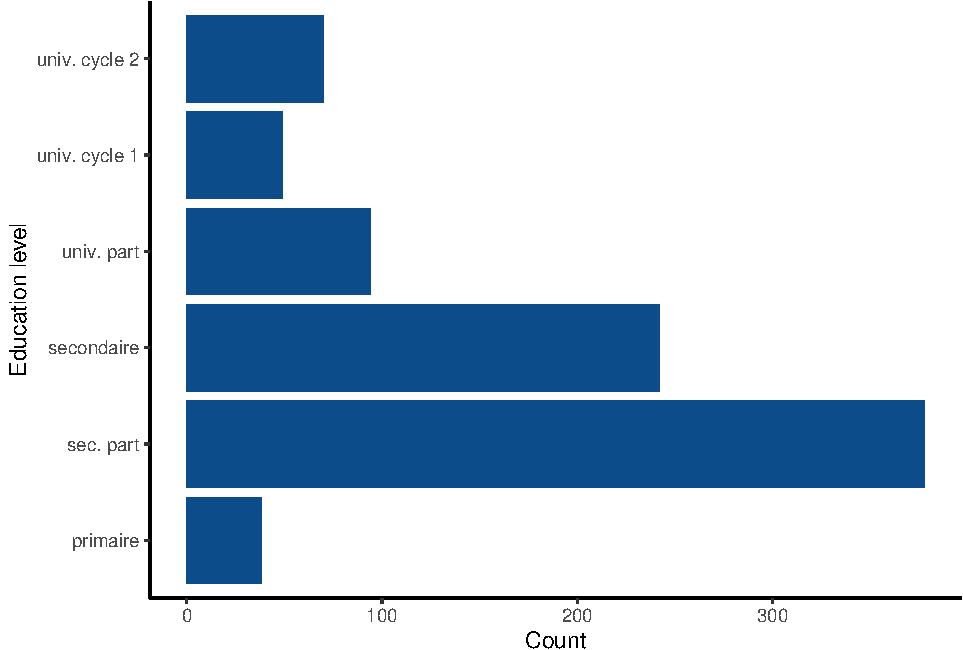
\includegraphics[width=1\linewidth]{perception_of_science_files/figure-latex/fig_edu-1} \caption{Distribution of respondants according to their education levels\label{fig:edu}.}\label{fig:fig_edu}
\end{figure}

Figure~\ref{fig:edu} presents the distribution of the sampled population
according to its education level. Quisque eleifend tincidunt ligula,
bibendum finibus massa cursus eget. Curabitur aliquet vehicula quam non
pulvinar. Aliquam facilisis tortor nec purus finibus, sit amet elementum
eros sodales. Ut porta porttitor vestibulum. Integer molestie, leo ut
maximus aliquam, velit dui iaculis nibh, eget hendrerit purus risus sit
amet dolor. Sed sed tincidunt ex. Curabitur imperdiet egestas tellus in
iaculis. Maecenas ante neque, pretium vel nisl at, lobortis lacinia
neque. In gravida elit vel volutpat imperdiet.

\hypertarget{question-b-and-education}{%
\subsection{Question B and education}\label{question-b-and-education}}

Lorem ipsum dolor sit amet, consectetur adipiscing elit. Aenean ut elit
odio. Donec fermentum tellus neque, vitae fringilla orci pretium vitae.
Fusce maximus finibus facilisis. Donec ut ullamcorper turpis. Donec ut
porta ipsum. Nullam cursus mauris a sapien ornare pulvinar. Aenean
malesuada molestie erat quis mattis. Praesent scelerisque posuere
faucibus. Praesent nunc nulla, ullamcorper ut ullamcorper sed, molestie
ut est. Donec consequat libero nisi, non semper velit vulputate et.
Quisque eleifend tincidunt ligula, bibendum finibus massa cursus eget.
Curabitur aliquet vehicula quam non pulvinar. Aliquam facilisis tortor
nec purus finibus, sit amet elementum eros sodales. Ut porta porttitor
vestibulum. Integer molestie, leo ut maximus aliquam, velit dui iaculis
nibh, eget hendrerit purus risus sit amet dolor. Sed sed tincidunt ex.
Curabitur imperdiet egestas tellus in iaculis. Maecenas ante neque,
pretium vel nisl at, lobortis lacinia neque. In gravida elit vel
volutpat imperdiet. Sed ut nulla arcu. Proin blandit interdum ex sit
amet laoreet. Phasellus efficitur, sem hendrerit mattis dapibus, nunc
tellus ornare nisi, nec eleifend enim nibh ac ipsum. Aenean tincidunt
nisl sit amet facilisis faucibus. Donec odio erat, bibendum eu imperdiet
sed, gravida luctus turpis.

Table~\ref{tab:b_edu} details the repartition of answers for question B
on whether science is more detrimental than benefic.

Lorem ipsum dolor sit amet, consectetur adipiscing elit. Aenean ut elit
odio. Donec fermentum tellus neque, vitae fringilla orci pretium vitae.
Fusce maximus finibus facilisis. Donec ut ullamcorper turpis. Donec ut
porta ipsum. Nullam cursus mauris a sapien ornare pulvinar. Aenean
malesuada molestie erat quis mattis. Praesent scelerisque posuere
faucibus. Praesent nunc nulla, ullamcorper ut ullamcorper sed, molestie
ut est. Donec consequat libero nisi, non semper velit vulputate et.
Quisque eleifend tincidunt ligula, bibendum finibus massa cursus eget.
Curabitur aliquet vehicula quam non pulvinar. Aliquam facilisis tortor
nec purus finibus, sit amet elementum eros sodales. Ut porta porttitor
vestibulum. Integer molestie, leo ut maximus aliquam, velit dui iaculis
nibh, eget hendrerit purus risus sit amet dolor. Sed sed tincidunt ex.
Curabitur imperdiet egestas tellus in iaculis. Maecenas ante neque,
pretium vel nisl at, lobortis lacinia neque. In gravida elit vel
volutpat imperdiet. Sed ut nulla arcu. Proin blandit interdum ex sit
amet laoreet. Phasellus efficitur, sem hendrerit mattis dapibus, nunc
tellus ornare nisi, nec eleifend enim nibh ac ipsum. Aenean tincidunt
nisl sit amet facilisis faucibus. Donec odio erat, bibendum eu imperdiet
sed, gravida luctus turpis.

A significant dependency between the answers to question B and the level
of education was found at \(\alpha\) level of 5\% (\(\chi^2\) test of
independence, \(\chi^2_{obs}\) = 42.76, df = 20, \emph{p}-value =
0.0022). The biplot for the first plane of a correspondance analysis
(Fig.~\ref{fig:b_edu}) shows that the lower the education, the more
respondant agree with question B

\begin{figure}
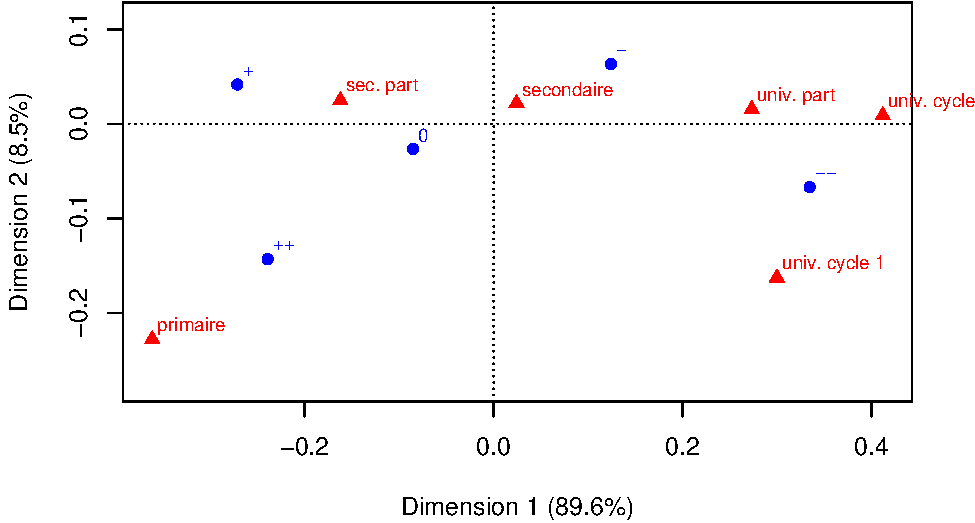
\includegraphics[width=1\linewidth]{perception_of_science_files/figure-latex/fig_b_edu-1} \caption{First plane of the correspondence analysis between answers to question B and education level\label{fig:b_edu}.}\label{fig:fig_b_edu}
\end{figure}

\hypertarget{question-d-and-education}{%
\subsection{Question D and education}\label{question-d-and-education}}

Question D is more ambiguous (Science will solve environment problems
without changing our way of life), and the answers are less clear. There
is no significant dependency at level \(\alpha\) = 5\% between answers
to question D and education level (\(\chi^2\) test of independence,
\(\chi^2_{obs}\) = 25.37, df = 20, \emph{p}-value = 0.1878).

Lorem ipsum dolor sit amet, consectetur adipiscing elit. Aenean ut elit
odio. Donec fermentum tellus neque, vitae fringilla orci pretium vitae.
Fusce maximus finibus facilisis. Donec ut ullamcorper turpis. Donec ut
porta ipsum. Nullam cursus mauris a sapien ornare pulvinar. Aenean
malesuada molestie erat quis mattis. Praesent scelerisque posuere
faucibus. Praesent nunc nulla, ullamcorper ut ullamcorper sed, molestie
ut est. Donec consequat libero nisi, non semper velit vulputate et.
Quisque eleifend tincidunt ligula, bibendum finibus massa cursus eget.
Curabitur aliquet vehicula quam non pulvinar. Aliquam facilisis tortor
nec purus finibus, sit amet elementum eros sodales. Ut porta porttitor
vestibulum. Integer molestie, leo ut maximus aliquam, velit dui iaculis
nibh, eget hendrerit purus risus sit amet dolor. Sed sed tincidunt ex.
Curabitur imperdiet egestas tellus in iaculis. Maecenas ante neque,
pretium vel nisl at, lobortis lacinia neque. In gravida elit vel
volutpat imperdiet. Sed ut nulla arcu. Proin blandit interdum ex sit
amet laoreet. Phasellus efficitur, sem hendrerit mattis dapibus, nunc
tellus ornare nisi, nec eleifend enim nibh ac ipsum. Aenean tincidunt
nisl sit amet facilisis faucibus. Donec odio erat, bibendum eu imperdiet
sed, gravida luctus turpis.

\hypertarget{discussion}{%
\section{Discussion}\label{discussion}}

Lorem ipsum dolor sit amet, consectetur adipiscing elit. Aenean ut elit
odio. Donec fermentum tellus neque, vitae fringilla orci pretium vitae.
Fusce maximus finibus facilisis. Donec ut ullamcorper turpis. Donec ut
porta ipsum. Nullam cursus mauris a sapien ornare pulvinar. Aenean
malesuada molestie erat quis mattis. Praesent scelerisque posuere
faucibus. Praesent nunc nulla, ullamcorper ut ullamcorper sed, molestie
ut est. Donec consequat libero nisi, non semper velit vulputate et.
Quisque eleifend tincidunt ligula, bibendum finibus massa cursus eget.
Curabitur aliquet vehicula quam non pulvinar. Aliquam facilisis tortor
nec purus finibus, sit amet elementum eros sodales. Ut porta porttitor
vestibulum. Integer molestie, leo ut maximus aliquam, velit dui iaculis
nibh, eget hendrerit purus risus sit amet dolor. Sed sed tincidunt ex.
Curabitur imperdiet egestas tellus in iaculis. Maecenas ante neque,
pretium vel nisl at, lobortis lacinia neque. In gravida elit vel
volutpat imperdiet. Sed ut nulla arcu. Proin blandit interdum ex sit
amet laoreet. Phasellus efficitur, sem hendrerit mattis dapibus, nunc
tellus ornare nisi, nec eleifend enim nibh ac ipsum. Aenean tincidunt
nisl sit amet facilisis faucibus. Donec odio erat, bibendum eu imperdiet
sed, gravida luctus turpis.

\hypertarget{author-contributions}{%
\section{Author Contributions}\label{author-contributions}}

Each author would like that the others have contributed more to this
manuscript!

\hypertarget{acknowledgments}{%
\section{Acknowledgments}\label{acknowledgments}}

The authors wish to thank the PerSciF FPSE UMONS for the opportunity to
submit these results.

\hypertarget{references}{%
\section*{References}\label{references}}
\addcontentsline{toc}{section}{References}

\hypertarget{refs}{}
\begin{CSLReferences}{1}{0}
\leavevmode\vadjust pre{\hypertarget{ref-Kamm2000}{}}%
Kamm, J. (2000). Evaluation of the {S}edov-von {N}eumann-{T}aylor blast
wave solution. Los {A}lamos {N}ational {L}aboratory.

\leavevmode\vadjust pre{\hypertarget{ref-Knupp1999}{}}%
Knupp, P. (1999). Winslow smoothing on two-dimensional unstructured
meshes. \emph{Eng {C}omput} 15, 263--268.

\leavevmode\vadjust pre{\hypertarget{ref-Taylor1937}{}}%
Taylor, G., and Green, A. (1937). Mechanism of the production of small
eddies from large ones. \emph{P {R}oy {S}oc {L}ond {A} {M}at} 158,
499--521.

\end{CSLReferences}

\begin{table}[ht]
\centering
\begin{tabular}{rrrrrrr}
  \hline
 & primaire & sec. part & secondaire & univ. part & univ. cycle 1 & univ. cycle 2 \\ 
  \hline
++ &   6 &  34 &  19 &   6 &   4 &   2 \\ 
  + &  10 &  93 &  47 &  12 &   5 &   7 \\ 
  0 &  11 &  95 &  55 &  18 &  11 &  15 \\ 
  - &   7 & 112 &  82 &  37 &  16 &  27 \\ 
  -- &   4 &  44 &  39 &  21 &  13 &  19 \\ 
   \hline
\end{tabular}
\caption{Repartition of answers to question B according to education level.} 
\label{tab:b_edu}
\end{table}


\end{document}
